Use this method to solve the initial value problem

$$
u'(t) = 2(t + 1),\; u(1) = 3.
$$

\begin{solution}\ \\\\
    \ \\
    For $f(t, U) = 2(t + 1)$, our implicit Runge-Kutta method with uniform grid spacing $k$ becomes:
    
    \begin{align*}
        Y_1 &= U^n + \frac{k}{2} \left[2\left(t_n + \frac{k}{2}\right) + 1 \right] \\ 
        U^{n+1} &= U^n + k\left[2\left(t_n + \frac{k}{2}\right) + 1 \right].
    \end{align*}
    
    We implement this in \texttt{problem\_3c.m} with \texttt{MATLAB} on the interval $t = [1, 5]$ with initial condition 
    $u(1) = 3$ and varying step sizes: \footnote{
        Note that the analytical solution to this ODE is given by $u(t) = t^2 + 2t$.
    }
    
    \begin{figure}[h]
        \centering
        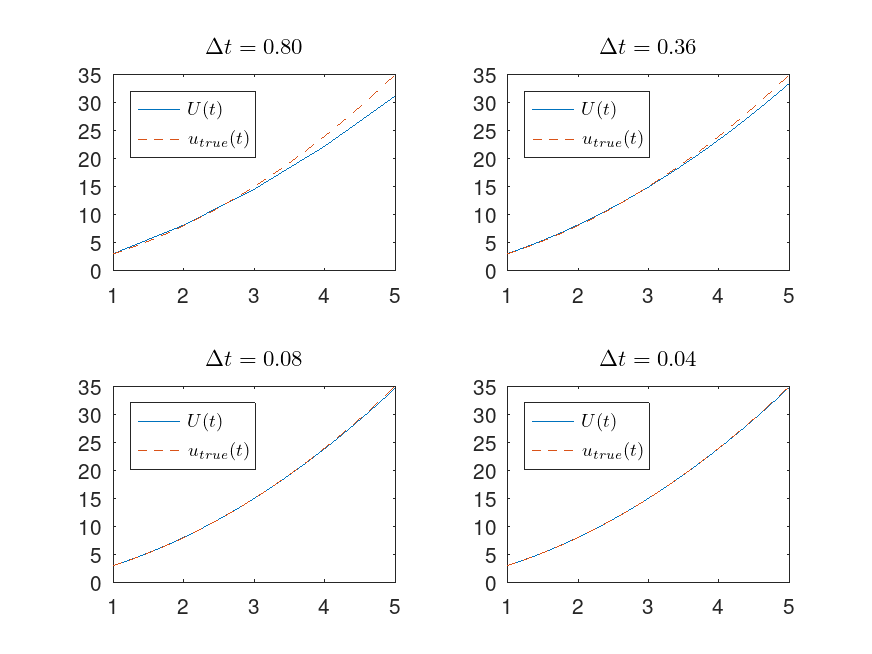
\includegraphics[width=0.85\textwidth]{problem_3c_solution.png}
        \caption[problem2b_solution]{Implicit RK solution to $u' = 2(t+1),\; u(1) = 3$}
    \end{figure}
\end{solution}